\documentclass[../p052main.tex]{subfiles}
\graphicspath{{\subfix{../figures/}}}

\begin{document}

\chapter{One-Dimensional Potentials}
\section{The Finite Square Well}
Now we'll look at a few different potentials $V(x)$ and determine what their corresponding wave functions look like.
Let's start with the finite square well:
\[ V(x) = \begin{cases} 0 & |x| < a/2, \\ V_0 & |x| > a/2. \end{cases} \]
We're interested in bound states, ones that satisfy $E < V_0$ (so that they're restricted to the well's interior).

The key difference between this arrangement and the infinite square well is that the particle \textit{can} exist in a state of finite energy.
It is now possible to detect the particle outside the bounds of our box, so our boundary conditions are going to change a bit.
We'll still require that $\psi$ be normalizable, so it must go to zero in its infinite limits.
It should also be continuous, but now that we're dealing with a finite potential, we also want $\psi$ to be smooth (so its first derivative is continuous).

We'll start by solving the Schrödinger equation as we did before.
On the left we have the inside of the well, and on the right the outside.
\begin{align*}
    -\frac{\hbar^2}{2m} \frac{d^2 \psi}{d x^2} &= E \psi & -\frac{\hbar^2}{2m} \frac{d^2 \psi}{d x^2} + V_0 \psi &= E \psi \\
    \frac{d^2 \psi}{dx^2} &= -\frac{2mE}{\hbar^2}\psi & \frac{d^2 \psi}{dx^2} &= \frac{2m(V_0 - E)}{\hbar^2} \psi \\
    \psi'' &= -k^2 \psi & \psi'' &= \kappa^2 \psi
\end{align*}
Here we've defined $k^2 \equiv 2mE/\hbar^2$ (as before) and $\kappa^2 \equiv 2m (V_0 - E)/\hbar^2$.
We can see that the inside of our well has complex exponential (or oscillatory) solutions, and the outside has real exponential solutions.
So we have the general solution
\[ \psi(x) = \begin{cases} C_1 e^{\kappa x} + C_2 e^{-\kappa x} & x < -a/2 \\ Ae^{ikx} + Be^{-ikx} & |x| < a/2 \\ D_1 e^{\kappa x} + D_2 e^{-\kappa x} & x > a/2 \end{cases} \]
But since $\psi$ must be normalizable, we can kill off a couple of divergent terms.
\[ \psi(x) = \begin{cases} C e^{\kappa x} & x < -a/2 \\ Ae^{ikx} + Be^{-ikx} & |x| < a/2 \\ D e^{-\kappa x} & x > a/2 \end{cases}
\implies
\frac{d\psi}{dx} = \begin{cases} \kappa Ce^{\kappa x} & x < -a/2 \\ ikAe^{ikx} - ikBe^{-ikx} & |x| < a/2 \\ -\kappa De^{-\kappa x} & x > a/2 \end{cases} \]
Now, to stitch these pieces together, we must ensure the continuity of $\psi$ and $\psi'$ at $x = -a/2$ and $x = a/2$.
\begin{align*}
    (1) \;\phantom{\kappa} Ce^{-\kappa a/2} &= Ae^{-ika/2} + Be^{ika/2} & (3) \hspace{4.5pt}\phantom{-\kappa} De^{-\kappa a/2} &= Ae^{ika/2} + Be^{-ika/2} \\
    (2) \; \kappa Ce^{-\kappa a/2} &= ikAe^{-ika/2} - ikBe^{ika/2} & (4) -\kappa De^{-\kappa a/2} &= ikA e^{ika/2} - ikBe^{-ika/2}
\end{align*}%<3 
We can eliminate $C$ from the equations by dividing $(1) / (2)$, and we remove $D$ by dividing $(3) / (4)$.
Solving each quotient for $A/B$ gives
\[ \frac{A}{B} = e^{ika} \left( \frac{\kappa + ik}{-\kappa + ik} \right) \,\text{ and }\; \frac{A}{B} = e^{-ika} \left( \frac{-\kappa + ik}{\kappa + ik} \right). \]
Multiplying these equations gives, simply, $(A / B)^2 = 1$!
So we have either $A = B$ and $A = -B$, in which cases (1) and (3) together show that $C = D$ or $C = -D$, respectively.
This gives us two different types of solutions:
\[ \psi(x) = \begin{cases} Ce^{\kappa x} & x < -a/2 \\ 2A \cos kx & |x| < a/2 \\
Ce^{-\kappa x} & x > a/2 \end{cases} \;\text{ and }\; \psi(x) = \begin{cases} -Ce^{\kappa x} & x < -a/2 \\ 2iA \sin kx & |x| < a/2 \\ Ce^{-\kappa x} & x > a/2 \end{cases} \]
Notice that the $\psi$ on the left is even while the $\psi$ on the right is odd.

At this point we still haven't quantized anything.
To change this, let's go back to dividing (1)/(2) and (3)/(4):
\begin{align*}
    \frac{ik}{\kappa} &= \frac{e^{-ika / 2} + e^{ika / 2}}{e^{-ika / 2} - e^{ika / 2}} & -\frac{ik}{\kappa} &= \frac{e^{ika / 2} - e^{-ika / 2}}{e^{ika / 2} + e^{-ika / 2}} \\
    &= \frac{\cos (ka / 2)}{-i \sin (ka / 2)} & &= \frac{i \sin (ka / 2)}{\cos (ka / 2)} \\
    \tan (ka / 2) &= \frac{\kappa a / 2}{ka / 2} & \cot (ka / 2) &= -\frac{\kappa a / 2}{ka / 2} \\
    \tan \xi &= \frac{\sqrt{\xi_0^2 - \xi^2}}{\xi} & -\cot \xi &= \frac{\sqrt{\xi_0^2 - \xi^2}}{\xi}
\end{align*}
Here we've defined the dimensionless variables
\[ \xi \equiv ka / 2 \;\text{ and }\; \xi_0 \equiv \frac{a}{\hbar} \sqrt{\frac{mV_0}{2}}. \]
Both of these equations are transcendental---in order to solve them, we must do so numerically or graphically.
Below we've provided a plot for each equation, in which the two sides of the equation are graphed against each other.
\begin{center}
    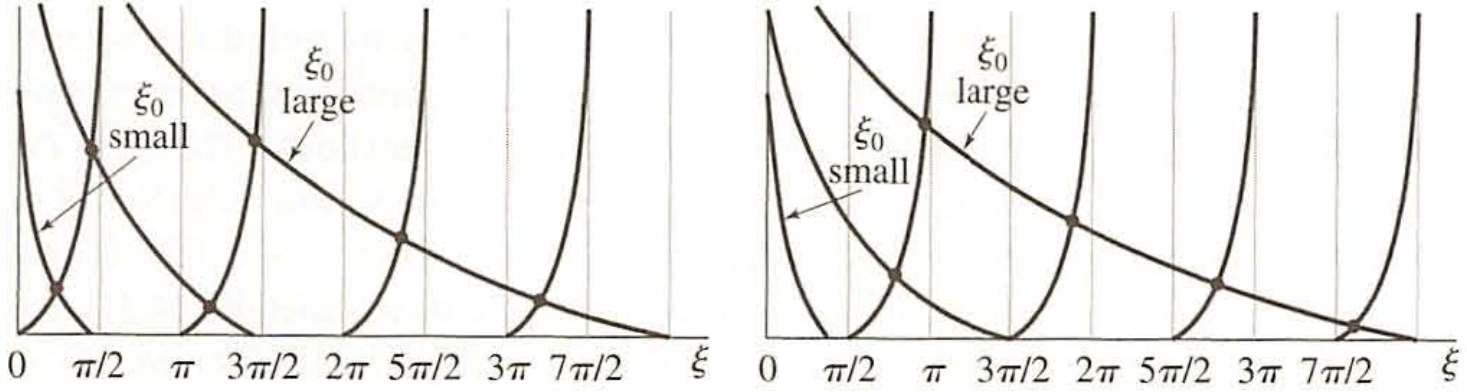
\includegraphics[width=0.75\textwidth]{fswPlots.png}
\end{center}
There are a few things to notice here.
First, each intersection corresponds to a distinct allowed $k$ and thus a distinct allowed energy, so our equations quantize the energy states of our wave functions!
There is also a finite number of energies this time, with a higher $\xi_0$ corresponding to more allowed energies.
This hopefully makes some intuitive sense: $\xi_0$ is a function of the well's size, and we'd expect that potential wells produce more bound states.
Finally, when we take the limit $V_0 \to \infty$, we get an infinite number of allowed energies determined by $\xi = n\pi / 2$ and we recover the infinite potential well energies, as we'd hope.

% \begin{summary}
%     The finite square well has oscillatory solutions on its interior and exponential ones on its exterior.
%     To determine precisely the behavior of these solutions, we apply continuity and differentiability boundary conditions, requiring that we eliminate any divergent terms which would otherwise ruin normalizability.
%     We eventually get a pair of equations that lack analytic solutions, but together they show that the allowed energies are once again quantized and that there are finitely many of them. 
% \end{summary}

\section{General Potential Wells}
Before moving on to other particular potentials, let's determine some qualitative characteristics of wave functions subject to potential wells in general.
%<3

Again, we're mostly interested in bound states.
For such a state there is a finite region for which $E > V$, which we'll call the classically bound region, and another for which $E < V$, which is classically forbidden.
Taking inspiration from the finite square well, we can rewrite the time-independent Schrödinger equation in convenient ways---one for $E > V$ and another for $E < V$.
\begin{align*}
    \frac{d^2 \psi}{d x^2} &= -\frac{2m[E - V(x)]}{\hbar^2} \psi & \frac{d^2 \psi}{d x^2} &= \frac{2m[V(x) - E]}{\hbar^2} \psi \\
    \frac{d^2 \psi}{d x^2} &= -k^2(x) \psi & \frac{d^2 \psi}{d x^2} &= \kappa^2(x) \psi
\end{align*}
These differential equations have oscillatory and exponential solutions, respectively.
\begin{itemize}[topsep=0pt]
    \item In the $E > V$ region the wave function will oscillate, and the frequency of oscillation increases as $E - V$ increases (i.e., as the potential energy $V$ decreases).
    If $E > V$ everywhere then we have a continuum of solutions that we can combine to create a normalizable wave packet, as we did before.

    \item In the $E < V$ region the wave function will be exponential, and the curve gets steeper as $V - E$ increases (as $V$ increases).
    If $E < V$ everywhere there are no physical solutions because $\psi$ will diverge and be non-normalizable.
\end{itemize}
If $E = V$ then $\psi''(x) = 0$ and we have an inflection point.
These are where we can apply continuity and differentiability boundary conditions to stitch together the exponential and oscillatory solutions.
This is also how energies get quantized---there are only so many energies that produce well-behaved, normalizable wave functions beyond these inflection points.
Each energy corresponds to a different number of half-oscillations; the $n$th bound state has $n-1$ nodes (zeroes).

At any particular point in the bound region, the wave function ``instantaneously'' looks like the sinusoid
\[ \psi(x) = A \sin (kx + \phi), \]
whose derivative is
\[ \frac{d\psi}{dx} = kA \cos (kx + \phi). \]
Suppose the potential $V$ abruptly rises at this point, so $k$ decreases; to maintain differentiability, the amplitude $A$ of the wave function must increase.
Thus there is an inverse relationship between $k$ and $A$, meaning the wave function has larger amplitudes in places with higher $V$.
This is perhaps counterintuitive from a classical standpoint since a higher potential energy corresponds to a lower kinetic energy and thus a lower amplitude, which goes to show how we can't lean so heavily on existing intuition here.

% \begin{summary}
%     Given a state with energy $E$, there are two key regions to consider.
%     \begin{itemize}
%         \item In the $E > V$ regions, solutions are oscillatory.
%         As $E-V$ increases, the frequency of oscillation increases and the amplitude decreases.
%         If $E > V$ everywhere then we have a continuum of solutions that we can combine to create a normalizable wave packet.
%         \item In the $E < V$ regions, solutions are exponential.
%         As $V-E$ increases, the ``decay length'' decreases.
%         If $E < V$ everywhere then there are no solutions because $\psi$ will diverge.
%     \end{itemize}
%     At $E = V$ we often see inflection points; this is where we apply continuity and differentiability boundary conditions to get quantized solutions and energies.
%     The $n$th bound state has $n-1$ nodes.
% \end{summary}

\section{The Quantum Harmonic Oscillator}
Recall, from Newtonian mechanics, that any smooth potential energy in the vicinity of a minimum looks like a harmonic oscillator and can be approximated by $V(x) \approx \frac{1}{2} kx^2$.
We can do something similar in quantum mechanics by solving the quantum harmonic oscillator,
\[ V(x) = \frac{1}{2}m \omega_0^2 x^2, \]
where $\omega_0^2 \equiv \frac{K}{m}$ and $K$ can be interpreted as the oscillator's ``effective spring constant''.
Like the particle in a box, we can solve for the exact energy eigenvalues and eigenfunctions, though it'll probably be less satisfying.
%<3

Let's gain our bearings by making a prediction about what the ground state energy should be.
For reasons that will soon become clear, let's call the ground-state eigenfunction $\psi_0$.
The expectation value of the corresponding energy is
\[ \left< E \right> = \frac{\left< p_x^2 \right>}{2m} + \frac{1}{2}m\omega_0^2 \left< x^2 \right>. \]
But since $\psi_0$ is a stationary state, the energy has a definite value $E_0$.
Also, since $\psi_0$ is an even, real function, $\left< x \right> = \left< p_x \right> = 0$.
So we can write
\[ E_0 = \frac{(\Delta p_x)^2}{2m} + \frac{1}{2}m\omega_0^2 (\Delta x)^2. \]
By the Heisenberg uncertainty principle,
\[ E_0 \geq \frac{\hbar^2}{8m (\Delta x)^2} + \frac{1}{2} m\omega_0^2 (\Delta x)^2. \]
Nature wants to minimize the energy in the ground state, so we differentiate the right side and set it equal to zero to get $(\Delta x)^2 = \hbar / 2m\omega_0$; substituting this back into our inequality,
\[ E_0 \geq \frac{1}{4} \hbar \omega_0 = \frac{1}{4} \hbar \omega_0 = \frac{1}{2} \hbar \omega_0. \]
So the absolute smallest energy a particle can have under the influence of the harmonic oscillator is $\hbar \omega_0 / 2$.
This is another profound departure from classical physics---our particle cannot just sit at rest at the bottom of our well because that would require knowing precisely both $\Delta x$ and $\Delta p_x$, which is impossible!

Armed with this preliminary result, we must now solve the time-independent Schrödinger equation
\[ \frac{d^2 \psi}{d x^2} = -\frac{2m}{\hbar^2} \left[ E - \frac{1}{2}m\omega_0^2x^2 \right] \psi. \]
This equation is nonlinear, which complicates things quite a bit.
To simplify things slightly, we can take the asymptotic limit as $x \to \pm \infty$ to get
\[ \frac{d^2 \psi}{d x^2} \approx \frac{m^2\omega_0^2x^2}{\hbar^2} \psi. \]
One can verify that an approximate solution for large $|x|$ is
\[ \psi_n(x) = x^{n} e^{-m\omega_0 x^2 / 2\hbar}, \]
where $n$ is a whole number.
In fact, if $n=0$, then this solution is exactly right for our original equation!
We can substitute $\psi_0$ to get the corresponding energy eigenvalue:
\begin{align*}
    \psi_0(x) &= A_0e^{-m\omega_0 x^2 / 2\hbar} \\
    H \psi_0(x) &= \frac{1}{2}\hbar\omega_0 \,\psi_0(x)
\end{align*}
Note, also, that $\psi_0$ must be the ground state since it has no nodes.
(So our indexing in this section will be slightly different from previous sections.)
We can normalize this function quite easily with a slick method using double integrals, shown below.

\begin{example}[Gaussian integral]
    Suppose we want to normalize the wave function $\psi_0(x) = A_0 e^{-m\omega_0 x^2 / 2\hbar}$.
    This requires solving the equation
    \begin{align*}
        1 &= \int_{-\infty}^{\infty} |A_0|^2 e^{-m\omega_0 x^2 / \hbar}dx \\
        \frac{1}{|A_0|^2} &= \int_{-\infty}^{\infty} e^{-b x^2}dx,
    \end{align*}
    where $b = m\omega_0 / \hbar$.
    Let's call the integral $\mathcal{I}$, so we can write
    \begin{align*}
        \mathcal{I}^2 &= \int_{-\infty}^{\infty} e^{-b x^2}dx \int_{-\infty}^{\infty} e^{-b y^2}dy \\
        &= \iint_{\mathbb{R}^2} e^{-b(x^2 + y^2)} dxdy.
        \intertext{Rewriting in polar form,}
        &= \int_0^{2\pi}\hspace{-5pt}\int_0^\infty e^{-br^2} r \,drd\theta \\
        \mathcal{I}^2 &= \frac{\pi}{b}
    \end{align*}
    So the normalization constant satisfies $|A_0| = (b / \pi)^{1/4}$.
\end{example}

One could use power series to generate more solutions to our Schrödinger equation, but for brevity's sake we won't do that here.
Instead we'll just quote the solution:
\[ \psi_n(x) = A_n H_n \left( \sqrt{\frac{m\omega_0}{\hbar}} x \right) e^{-m\omega_0x^2 / 2\hbar}, \]
where $H_n$ is the $n$th degree Hermite polynomial.
Plotting these solutions shows that they have all the characteristics we'd expect from the previous section!
They're oscillatory with increasing amplitude up to a point, after which they decay exponentially to zero.
The corresponding energy eigenvalues are
\[ E_n = \left( n + \frac{1}{2} \right) \hbar \omega_0. \]
Now, each $\psi_n$ is a stationary state.
Their magnitudes do not evolve in time.
However, there \textit{is} a linear combination of these states that exhibits the same kind of oscillatory behavior we'd expect from a classical standpoint, which is pretty cool!

% \begin{summary}
%     According to the Heisenberg uncertainty principle, the quantum harmonic oscillator must have a nonzero minimum allowed energy.
%     In particular, $E_0 = \hbar \omega_0 / 2$, and $\psi_0(x) = A_0 e^{-m \omega_0 x^2 / 2\hbar}$.
%     The other energies are evenly-spaced up the potential well, but their associated eigenfunctions take a more complex form involving Hermite polynomials.
% \end{summary}

\section{Delta Function Potentials}
We'll look at a new potential in this section, but first, let's talk about the Dirac delta function.
Firstly, the word ``function'' is an incredible misnomer---the Dirac delta function is not a function at all, but rather a distribution that only has meaning when integrated over.
If we define it as the limit of normalized Gaussians,
\[ \delta (x) = \lim_{b \to \infty} \sqrt{\frac{b}{\pi}} e^{-bx^2} = \begin{cases} 0 & x \neq 0 \\ \infty & x = 0 \end{cases}, \]
then the integral over a delta spike is one.
Thus %<3
\[ \int_{-\infty}^{\infty} f(x) \delta(x) \,dx = f(0) \int_{-\infty}^{\infty} \delta(x) \,dx = f(0), \]
which we'll take advantage of plenty later.
As a side note, notice that we can write
\[ f(x) \,\delta (x - x_0) = f(x_0) \,\delta (x - x_0), \]
and that we can substitute $f(x) = x$ to get
\[ x \,\delta (x - x_0) = x_0 \,\delta (x - x_0). \]
This is an eigenvalue equation for the position operator!
So $\delta (x - x_0)$ is an eigenfunction and $x_0$ its eigenvalue.

Anyway, now we'll consider the point potential
\[ V(x) = -\frac{\hbar^2 \alpha}{2ma} \delta(x), \]
where $\alpha$ is dimensionless and tells us about the strength of the potential, and $a$ is some other constant with units of length.
(The unitless space integral of $\delta$ implies that $\delta$ has units of inverse length.)
In order for a state to be bound in this potential it must have $E < 0$, so on either side of the origin we have $E < V$.
This gives the time-independent Schrödinger equation
\[ \frac{d^2 \psi}{d x^2} = -\frac{2mE}{\hbar^2} \psi \implies \frac{d^2 \psi}{d x^2} = \kappa^2 \psi, \]
the solution of which is
\[ \psi(x) = \begin{cases} Ae^{\kappa x} & x < 0, \\ Be^{-\kappa x} & x > 0, \end{cases} \]
as expected based on our qualitative understanding of wave functions.
Now let's apply the boundary conditions.
Since $\psi$ is continuous, $A = B$.
But since we have an infinity here, $\psi$ need not be differentiable.
We can still determine a relationship between the one-sided derivatives at $x=0$.
First, we have the time-independent Schrödinger equation
\begin{align*}
    \frac{d^2 \psi}{d x^2} &= \frac{2m}{\hbar^2} \left( V(x) - E \right) \psi \\
    \frac{d}{dx} \frac{d\psi}{dx} &= \frac{2m}{\hbar^2} \left( -\frac{\hbar^2 \alpha}{2ma} \delta(x) - E \right) \psi(x)
\end{align*}
We want to determine what happens to $\psi'$ as we move across $x=0$, so let's integrate over a small neighborhood of 0 and see what happens!
\begin{align*}
    \int_{-\epsilon}^{\epsilon} \frac{d}{dx} \frac{d\psi}{dx} \,dx &= \int_{-\epsilon}^{\epsilon} \frac{2m}{\hbar^2} \left( -\frac{\hbar^2 \alpha}{2ma} \delta(x) - E \right) \psi(x) \,dx \\
    \frac{d\psi}{dx} \Big|_{-\epsilon}^\epsilon &= -\frac{\alpha}{a} \int_{-\epsilon}^{\epsilon} \delta(x) \psi(x) \,dx - \frac{2mE}{\hbar^2} \int_{-\epsilon}^{\epsilon} \psi(x) \,dx \\
    \intertext{Taking the limit as $\epsilon \to 0$:}
    \frac{d\psi}{dx}\Big|_{0^-}^{0^+} &= -\frac{\alpha}{a}\psi(0)
\end{align*}
This is our boundary condition for differentiability.
To apply it, let's take the derivative of our wave function.
\[ \psi(x) = \begin{cases} \kappa Ae^{\kappa x} & x < 0, \\ -\kappa Ae^{-\kappa x} & x > 0, \end{cases} \]
So we must have
\begin{align*}
    -\kappa Ae^{-\kappa \cdot 0} - \kappa A e^{\kappa \cdot 0} &= -\frac{\alpha}{a}\psi(0) \\
    -\kappa \psi(0) - \kappa \psi(0) &= -\frac{\alpha}{a}\psi(0)
\end{align*}
So $\kappa = \frac{\alpha}{2a}$, which corresponds to $E = -(\hbar^2 \alpha^2) / (8ma^2)$.
This is the only possible energy level!
%<3

Closely related to this is the double delta well.
We'll skim over the details, but in general we have
\[ V(x) = -\frac{\hbar^2 \alpha}{2ma} \left[ \delta (x-a) + \delta (x+a) \right], \]
and by noting that the ground-state wave function is even we get
\[ \psi_0(x) = \begin{cases} Ce^{\kappa x} & x < -a, \\ A \cosh (\kappa x) & |x| < a, \\ Ce^{-\kappa x} & x > a. \end{cases} \]
When we impose the continuity and differentiability boundary conditions we get
\[ \tanh (\kappa a) = \frac{\alpha}{\kappa a} - 1. \]
This is another transcendental equation, but since $\tanh (\kappa a)$ we'll always have
\[ \frac{\alpha}{\kappa a} - 1 < 1 \implies E < -\frac{\hbar^2 \alpha^2}{8ma^2}. \]
So this double well is more tightly bound than the single well!
Interpreted as a crude model for diatomic molecules, this explains why molecules are more stable than individual atoms.

% \begin{summary}
%     The Dirac delta potential has exponential solutions on either side of the spike.
%     These solutions piece together to create a continuous solution.
%     There is also a differentiability boundary condition that is uncovered by integrating either side of the Schrödinger equation over an infinitesimal neighborhood around the potential spike.
%     If we do a similar thing with a double delta well we get a solution that is more tightly bound (i.e., one that has a lower energy).
% \end{summary}

\section{Quantum Scattering}
Now we'll step into the world of unbound states, which have continuous energy eigenvalues and non-normalizable energy eigenfunctions.
While we study the potentials of bound states using spectroscopy, we use scattering to study those of unbound states.

To simplify things, we'll just talk about the step potential:
\[ V(x) = \begin{cases} 0 & x < 0 \\ V_0 & x > 0 \end{cases} \]
Suppose a particle with $E > V_0$ travels to the right and is incident on the step.
The corresponding wave function will have a reflected component and a transmitted component.
To see the specifics of how this works, let's once again go through the process of solving the Schrödinger equation.
In the left and right regions we have, respectively,
\begin{align*}
    \psi'' &= -k^2 \psi, & \psi'' &= -k_0^2 \psi, \\
    k^2 &= \frac{2mE}{\hbar^2}, & -k_0^2 &= \frac{2m(E - V_0)}{\hbar^2}.
\end{align*}
This yields the wave function
\[ \psi(x) = \begin{cases} Ae^{ikx} + Be^{-ikx} & x < 0 \\ Ce^{ik_0x} + De^{-ik_0x} & x > 0 \end{cases} \;\implies\; \psi'(x) = \begin{cases} ik(Ae^{ikx} - Be^{-ikx}) & x < 0 \\ ik_0(Ce^{ik_0x} - De^{-ik_0x}) & x > 0 \end{cases} \]
The continuity of $\psi$ and its derivative require that
\begin{align*}
    A + B &= C + D \\
    ik(A - B) &= ik_0(C - D)
\end{align*}
For any individual $k$ we won't get a solution that's normalizable, so they can't give us any absolute probabilities.
But we can appeal to the probability current to determine what fraction of the incident probability is reflected and transmitted!
It's straightforward to show that
\[ j_x = \begin{cases} \frac{\hbar k}{m} \left( |A|^2 - |B|^2 \right) & x < 0, \\ \frac{\hbar k_0}{m} \left( |C|^2 - |D|^2 \right) & x > 0. \end{cases} \]
Looking back at our wave function, we might interpret $|A|$ as describing the amount of probability on the left side of $x=0$ that flows in the $+x$ direction (the incident probability) and $|B|$ as that in the $-x$ (the transmitted).
So we can break the probability current into two parts:
\[ j_L = j_\textrm{inc} - j_\textrm{ref}. \]
We can do a similar analysis in the right region.
Notice, though, that we must set $D = 0$ because the particle enters the region from the left and can only travel rightward.
We can use this to simplify our boundary conditions:
\begin{align*}
    A + B &= C \\
    k(A - B) &= k_0 C
\end{align*}
This leads us to $C = [2k / (k + k_0)] A$ and $B = [(k - k_0) / (k + k_0)]A$.
So the reflection and transmission coefficients are
\[ R = \frac{j_\textrm{ref}}{j_\textrm{inc}} = \frac{|B|^2}{|A|^2} = \left( \frac{k - k_0}{k + k_0} \right)^2, \qquad T = \frac{j_\textrm{trans}}{j_\textrm{inc}} = \frac{k_0}{k} \frac{|C|^2}{|A|^2} = \frac{4kk_0}{(k + k_0)^2}. \]
Now, what if $E < V_0$?
In this case the left region is the same as before, but on the right we have the time-independent Schrödinger equation
\[ \psi'' = \kappa \psi, \qquad \kappa^2 = \frac{2m(V_0 - E)}{\hbar^2}. \]
The solution of this equation is real-valued, meaning its probability current is zero.
So there is no transmitted probability and the reflection coefficient is one!
(Note that there is still a decaying probability of detection beyond the step---this probability just doesn't ``propagate''.)

% \begin{summary}
%     When a wave function is incident on some sudden step in potential satisfying $V_0 < E$, some probability is transmitted through the step and the rest is reflected.
%     These amounts are quantified by the reflection and transmission coefficients
%     \[ R = \frac{j_\textrm{ref}}{j_\textrm{inc}}, \qquad T = \frac{j_\textrm{trans}}{j_\textrm{inc}}, \]
%     where each $j$ is the relevant component of the probability current.
%     When $V_0 > E$, the region within the potential step has no probability current because the wave function is real-valued there.
% \end{summary}

\section{Quantum Tunneling}
Now consider the finite barrier
\[ V(x) = \begin{cases} V_0 & 0 < x < a \\ 0 & \textrm{elsewhere} \end{cases} \]
If a particle has energy $E > V_0$ then we'll still get reflection and transmission, it'll just happen locally at each ``interface''.
What we're really interested in is the $E < V_0$ case!

In the left, center, and right regions we have the respective time-independent Schrödinger equations
\[ \frac{d^2 \psi}{d x^2} = -k^2 \psi, \quad \frac{d^2 \psi}{d x^2} = \kappa^2 \psi, \quad \frac{d^2 \psi}{d x^2} = -k^2 \psi, \]
where $k^2$ and $\kappa^2$ are defined in the familiar ways.
This gives the wave function
\[ \psi(x) = \begin{cases} Ae^{ikx} + Be^{-ikx} & x < 0, \\ Fe^{\kappa x} + Ge^{-\kappa x} & 0 < x < a, \\ Ce^{ikx} & x > a, \end{cases} \]
where the decaying term in the third region is omitted because, as before, there is no probability coming in from the right here.
Now we'll apply the continuity and differentiability boundary conditions:
\begin{align*}
    A + B &= F + G & Fe^{\kappa a} + Ge^{-\kappa a} &= Ce^{ika} \\
    ik (A - B) &= \kappa (F - G) & \kappa (Fe^{\kappa a} - Ge^{-\kappa a}) &= ik C e^{ika}
\end{align*}
From here we could show, with some nasty algebra, that the transmission coefficient through the barrier is
\[ T = \frac{k_\textrm{trans}}{k_\textrm{inc}} \frac{|C|^2}{|A|^2} = \left[ 1 + \frac{(k^2 + \kappa^2)^2}{4k^2\kappa^2} \sinh^2 (\kappa a) \right]^{-1}. \]
To make some sense of this expression, let's consider the limits as the barrier gets very thin ($\kappa a \ll 1$) or very thick ($\kappa a \gg 1$).
In the thin limit $\sinh^2 \kappa a \approx \kappa^2 a^2$ is negligibly small, so
\[ T_\textrm{small} \approx 1. \]
In the thick limit, though, $\sinh^2 \kappa x \approx e^{2\kappa a} / 2$, which is much larger than the constant term.
This gives
\[ T_\textrm{big} \approx \left( \frac{4k \kappa}{k^2 + \kappa^2} \right)^2 e^{-2\kappa a}. \]
Both of these should, hopefully, make some intuitive sense!
We'd expect most particles to tunnel through a very thin barrier, and based on our qualitative understanding of wave functions, the probability of tunneling should decay exponentially with thicker barriers.

We can easily extend our analysis to non-rectangular barriers by breaking it into a series of ``thick'' rectangular barriers, each with transmission coefficient
\[ T_j = C_j(k) \exp [-2 \kappa (x_j) \Delta x], \]
where $C_j(k)$ is some (constant) polynomial in $k$.
If we use $N$ pieces then the total transmission coefficient is approximately
\[ T \approx \prod_{j=1}^{N} T_j \propto \exp \left[ -2 \sum_{j=1}^{N} \kappa (x_j) \Delta x \right]. \]
In the limit, this turns into
\[ T \propto \exp \left[ -2 \int_{a}^{b} \kappa (x) \,dx \right] = \exp \left[ -\frac{2\sqrt{2m}}{\hbar} \int_{a}^{b} \sqrt{V(x) - E} \,dx \right], \]
where the constant of proportionality is some other polynomial in $k$.

% \begin{summary}
%     When a wave function is incident on a potential barrier (rather than a simple step) satisfying $V_0 > E$, then there is some transmitted probability.
%     Using the same analysis as before, we can find that the transmission coefficient through the barrier goes to 1 in the thin limit and to 0 in the thick limit.
% \end{summary}

\end{document}

%<3
%<3